%! Author = Juniell
%! Date = 08.05.2021

% Preamble
\documentclass[a4paper, 14pt]{extarticle}

% Packages
\usepackage[T2A]{fontenc}
\usepackage{natbib}
\usepackage{graphicx}
\usepackage[english, russian]{babel}
\usepackage{fontspec}
\usepackage{amsmath}
\usepackage{amsfonts}
\usepackage{amssymb}
\usepackage{amsthm}
\usepackage{mathtools}
\usepackage{mathrsfs}
\usepackage{fullpage}
\usepackage{ulem}
\usepackage{setspace}
\usepackage{listings}
\usepackage{indentfirst}
\usepackage[left=2cm,right=1.5cm,top=2cm,bottom=2cm]{geometry}
\usepackage{xcolor}
\usepackage{float}
\usepackage{csquotes}
\usepackage{hyperref}
\usepackage{graphics}

\definecolor{urlcolor}{HTML}{0000FF} % цвет ссылок
\definecolor{linkcolor}{HTML}{000000} % цвет гиперссылок
\hypersetup{pdfstartview=FitH, linkcolor=linkcolor, urlcolor=urlcolor, colorlinks=true}

\setmainfont{Times New Roman}
\setlength{\parindent}{5ex}
\setlength{\parskip}{1em}
\renewcommand{\baselinestretch}{1}

\graphicspath{{resources/Images}}

\definecolor{buzzlightyear}{HTML}{8757A5}
\definecolor{grass}{HTML}{738D06}
\definecolor{literal}{HTML}{F18A2B}
\definecolor{commentcolor}{HTML}{8E908B}

\lstdefinestyle{habrstyle}{
    backgroundcolor=\color{white},
    commentstyle=\color{commentcolor},
    keywordstyle=\bfseries\color{buzzlightyear},
    numberstyle=\tiny\color{commentcolor},
    stringstyle=\color{grass},
    basicstyle=\ttfamily\footnotesize,
    breakatwhitespace=false,
    breaklines=true,
    captionpos=b,
    keepspaces=true,
    numbers=left,
    numbersep=5pt,
    showspaces=false,
    showstringspaces=false,
    showtabs=false,
    tabsize=4,
    language=Python
}

\lstset{style=habrstyle}


% Document
\begin{document}
% Титульный лист
    \begin{center}
        \begin{center}
            \hfill \break
            \normalsize{Санкт-Петербургский государственный политехнический}\\
            \normalsize{университет Петра Великого}\\
            \hfill \break
            \normalsize{\textbf{Высшая школа интеллектуальных систем и}}\\
            \normalsize{\textbf{суперкомпьютерных технологий}}\\
            \hfill \break
            \hfill \break
            \hfill \break
            \hfill \break
            \hfill \break
            \normalsize{Отчёт по лабораторной работе №5}\\
            \normalsize{Дисциплина: Телекоммуникационные технологии}\\
            \normalsize{Тема: Автокорреляция}\\
        \end{center}
        \hfill \break
        \hfill \break
        \hfill \break
        \hfill \break
        \hfill \break
        \hfill \break
        \hfill \break
        \hfill \break
        \hfill \break
        \hfill \break
        \begin{tabbing}
            Выполнил студент гр. 3530901/80201 \`В.А. Пучкина\\
            \\
            Преподаватель: \`Н.В. Богач\\
        \end{tabbing}
        \hfill \break
        \hfill \break
        \hfill \break
        \hfill \break
        \begin{center}
            Санкт-Петербург\\
            2021
        \end{center}
        \thispagestyle{empty}
    \end{center}

% Оглавление
    \newpage
    \tableofcontents

% Список иллюстраций
    \newpage
    \listoffigures

% Список листингов
    \newpage
    \lstlistoflistings

% ---------------------------------------------- Упражнение 5.1 ----------------------------------------------
    \newpage
    \section{Упражнение 5.1}
    \label{sec:task1}

    Это упражнение направлено на знакомство с вычислением автокорреляции.
    Необходимо на основе информации из файла \texttt{chap05.ipynb} оценить высоты тона вокального \texttt{chirp}
    для нескольких времён начала сегмента.

    Сначала определим методы, описанные в \texttt{chap05.ipnyb}.

    \begin{lstlisting}[caption= Методы \texttt{serial\_corr} и \texttt{autocorr}., label={lst:task1_function}]
def serial_corr(wave, lag=1):
    N = len(wave)
    y1 = wave.ys[lag:]
    y2 = wave.ys[:N-lag]
    corr = numpy.corrcoef(y1, y2)[0, 1])
    return corr

def autocorr(wave):
    lags = numpy.arange(len(wave.ys)//2)
    corrs = [serial_corr(wave, lag) for lag in lags]
    return lags, corrs      \end{lstlisting}

    Теперь считаем файл с вокальным \texttt{chirp} и выберем сегмент.

    \begin{lstlisting}[caption= Чтение файла и выбор сегмента., label={lst:task1_read}]
voice_wave = read_wave('resources/Sounds/task1_bcjordan__voicedownbew.wav')
voice_wave.normalize()
voice_segment = voice_wave.segment(start=0.3, duration=0.01)
voice_wave.make_audio() \end{lstlisting}

    Получим автокорреляционную функцию выбранного сегмента с помощью \texttt{autocorr}.

    \begin{lstlisting}[caption= Получение автокорреляционной функции выбранного сегмента., label={lst:task1_autocorr_1}]
lag, corrs = autocorr(voice_segment)
plt.plot(lag, corrs)
decorate(xlabel='Lag', ylabel='Correlation')    \end{lstlisting}

    Из Рис.\ref{fig:task1_autocorr_1} видно, что первый пик находится примерно при lag = 110.
    Найдем точный индекс и определим частоту.

    \begin{lstlisting}[caption= Поиск пика и вычисление его частоты., label={lst:task1_freq_1}]
lag = numpy.array(corrs[100:130]).argmax() + 100
period = lag / voice_segment.framerate
freq = 1 / period
print("lag =", lag, "\nfreq =", freq)   \end{lstlisting}

    \begin{figure}[H]
        \centering
        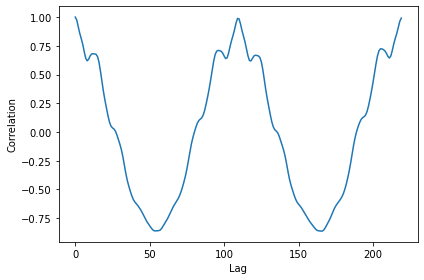
\includegraphics[width=0.8\linewidth]{resources/Images/task1_autocorr_1}
        \caption{Автокорреляционная функция для выбранного сегмента.}
        \label{fig:task1_autocorr_1}
    \end{figure}

    Были получены следующие результаты: lag = 109, частота = 404.6.
    Теперь выберем следующий сегмент и проделаем с ним те же действия.

    \begin{lstlisting}[caption= Получение автокорреляционной функции второго сегмента., label={lst:task1_segment_2}]
voice_segment = voice_wave.segment(start=0.7, duration=0.01)
lag, corrs = autocorr(voice_segment)
plt.plot(lag, corrs)
decorate(xlabel='Lag', ylabel='Correlation')    \end{lstlisting}

    На Рис.\ref{fig:task1_autocorr_2} видно, что первый пик находится примерно при lag = 130.
    Найдем точный индекс и определим частоту.

    \begin{lstlisting}[caption= Поиск пика и вычисление его частоты., label={lst:task1_freq_2}]
lag = numpy.array(corrs[120:140]).argmax() + 120
period = lag / voice_segment.framerate
freq = 1 / period
print("lag =", lag, "\nfreq =", freq)   \end{lstlisting}

    Были получены следующие результаты: lag = 127, частота = 347.2.
    Таким образом, частота вокального \texttt{chirp} уменьшается с течением времени.

    \begin{figure}[H]
        \centering
        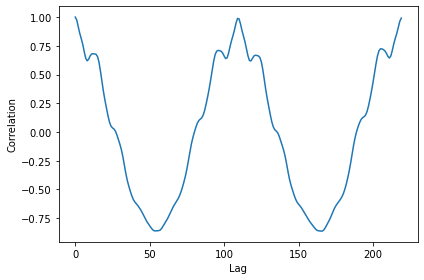
\includegraphics[width=0.8\linewidth]{resources/Images/task1_autocorr_1}
        \caption{Автокорреляционная функция для выбранного сегмента.}
        \label{fig:task1_autocorr_2}
    \end{figure}

    В ходе данного упражнения был получены автокорреляционные функции для двух сегментов записи вокального \texttt{chirp}.
    На них были выделены пики и получены их частоты.
    Был сделан вывод, что частота этого вокального \texttt{chirp} уменьшается с течением времени.

    \newpage

% ---------------------------------------------- Упражнение 5.2 ----------------------------------------------
    \section{Упражнение 5.2}
    \label{sec:task2}

    В этом упражнении необходимо выделить в отдельную функцию с названием \texttt{estimate\_fundamental} код из
    \texttt{chap05.ipnyb}, использующий автокорреляцию для оценки основной частоты периодического сигнала.
    Затем следует использовать эту функцию для отслеживания высоты тона записанного звука и проверить качество её работы,
    накладывая оценки высоты тона на спектрограмму записи.

    Итак, выделим необходимый код в функцию \texttt{estimate\_fundamental}.

    \begin{lstlisting}[caption= Функция \texttt{estimate\_fundamental}., label={lst:task2_fun}]
def estimate_fundamental(wave, low = 50, high = 150):
    lags, corrs = autocorr(wave)
    lag = numpy.array(corrs[low:high]).argmax() + low
    period = lag / wave.framerate
    freq = 1 / period
    return freq     \end{lstlisting}

    Теперь проверим работу этой функции на примере записи из \S\,\ref{sec:task1}.
    Для этого используем это функцию и будем накладывать её оценки высоты тона на спектрограмму записи.

    Сначала посмотрим на спектрограмму записи.

    \begin{lstlisting}[caption= Полуение спектрограммы., label={lst:task2_spectrogram}]
voice_wave.make_spectrogram(2048).plot(5000)
decorate(xlabel='Time (s)', ylabel='Frequency (Hz)')    \end{lstlisting}

    \begin{figure}[h]
        \centering
        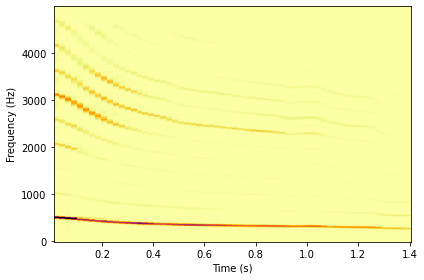
\includegraphics[width=0.7\linewidth]{resources/Images/task2_spectrogram}
        \caption{Спектрограмма записи.}
        \label{fig:task2_spectrogram}
    \end{figure}

    Теперь используем написанную функцию для получения оценок высоты.

    \begin{lstlisting}[caption= Полуение оценок высоты тона., label={lst:task2_grades}]
ts = []
freqs = []
step = 0.05
starts = numpy.arange(0.0, 1.4, step)

for start in starts:
    ts.append(start + step / 2)
    segment = voice_wave.segment(start=start, duration=0.01)
    freq = estimate_fundamental(segment)
    freqs.append(freq)  \end{lstlisting}

    Теперь нанесём полученные оценки на спектрограмму и посмотрим на результат.

    \begin{lstlisting}[caption= Сравнение полученных оценок со спектрограммой., label={lst:task2_grades_spectrogram}]
voice_wave.make_spectrogram(2048).plot(1000)
plt.plot(ts, freqs, color='white')
decorate(xlabel='Time (s)', ylabel='Frequency (Hz)')    \end{lstlisting}

    Из полученный спектрограммы (Рис.\ref{fig:task2_grades_spectrogram}) видно, что \texttt{estimate\_fundamental}
    выдаёт корректные оценки основной частоты периодического сигнала.

    \begin{figure}[H]
        \centering
        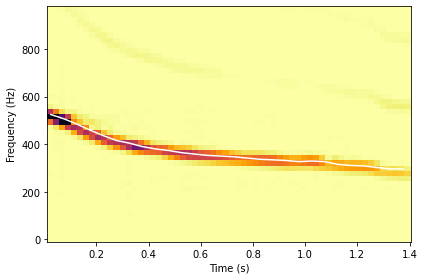
\includegraphics[width=0.7\linewidth]{resources/Images/task2_grades_spectrogram}
        \caption{Спектрограмма тона с наложенными оценками (белая линия).}
        \label{fig:task2_grades_spectrogram}
    \end{figure}

    В ходе выполнения данного упражнения на основе кода из \texttt{chap05.ipnyb} была написана функция \texttt{estimate\_fundamental}
    для оценки основной частоты периодического сигнала. Она также была протестирована на записи вокального \texttt{chirp}
    для отслеживания высоты тона записанного звука. После чего полученные оценки высоты тона были наложены на спектрограмму.
    Из полученного результата был сделан вывод, что написанная функция работает корректно.

    \newpage

% ---------------------------------------------- Упражнение 5.3 ----------------------------------------------
    \section{Упражнение 5.3}
    \label{sec:task3}

    В данном упражнении необходимо использовать данные о курсе BitCoin из 4 лабораторной работы для вычисления
    автокорреляции цен BitCoin.

    Итак, считаем файл и преобразуем данные в \texttt{wave}.

    \begin{lstlisting}[caption= Чтение файла и получение \texttt{wave}., label={lst:task3_wave_btc}]
df = pandas.read_csv('resources/task3_BTC_USD_2013-10-01_2021-05-07.csv', parse_dates=[0])
ys = df['Closing Price (USD)']
ts = df.index

wave_btc = Wave(ys, ts, framerate=1)
wave_btc.plot()
decorate(xlabel='Time (days)', ylabel='Price of BitCoin ($)')   \end{lstlisting}

    \begin{figure}[h]
        \centering
        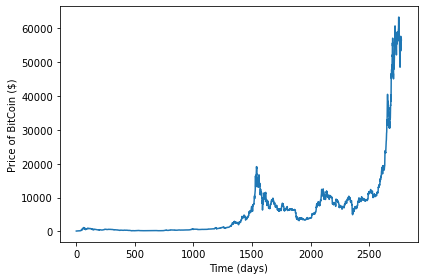
\includegraphics[width=0.8\linewidth]{resources/Images/task3_wave_btc}
        \caption{Курс BitCoin.}
        \label{fig:task3_wave_btc}
    \end{figure}

    Теперь получим автокорреляционную функцию и рассмотрим её.

    \begin{lstlisting}[caption= Получение автокорреляционной функции для курса BitCon., label={lst:task3_autocorr_btc}]
lag, corrs = autocorr(wave_btc)
plt.plot(lag, corrs)
decorate(xlabel='Lag', ylabel='Correlation')    \end{lstlisting}

    По полученному графику (Рис.\ref{fig:task3_autocorr_btc}) видно, что автокорреляционная функция не имеет периодичности.
    Кроме того, она имеет как спады, так и подъёмы.

    \begin{figure}[H]
        \centering
        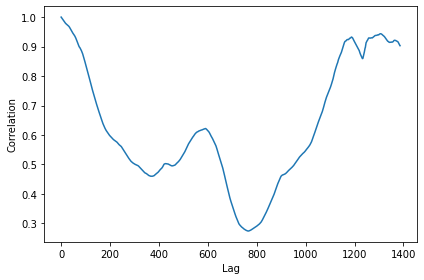
\includegraphics[width=0.8\linewidth]{resources/Images/task3_autocorr_btc}
        \caption{Автокорреляционная функция курса BitCoin.}
        \label{fig:task3_autocorr_btc}
    \end{figure}

    В ходе выполнения данного упражнения был проведён эксперимент с курсом BitCoin. На основе курса была получена
    \texttt{wave}, после чего вычислена автокорреляционная функция. Был сделан вывод, что автокорреляционная функция
    курса BitCoin не периодическая и имеет как спады, так и падения.

    \newpage

% ---------------------------------------------- Упражнение 5.4 ----------------------------------------------
    \section{Упражнение 5.4}
    \label{sec:task4}

    В данном упражнении необходимо изучить файл \texttt{saxophone.ipynb} и <<погонять>> примеры. В этом файле исследуются
    автокорреляция, восприятие высоты тона и явление <<подавленная основная>>.
    После изучения примеров следует выбрать другой сегмент записи и вновь поработать с ним.

    Итак, для начала считаем файл и получим его спектрограмму.

    \begin{lstlisting}[caption= Чтение файла и получение спектрограммы., label={lst:task4_spectrogram}]
sax_wave = read_wave('resources/Sounds/task4_iluppai__saxophone_weep.wav')
sax_wave.normalize()
sax_wave.make_spectrogram(seg_length=1024).plot(high=3000)
decorate(xlabel='Time (s)', ylabel='Frequency (Hz)')
sax_wave.make_audio()   \end{lstlisting}

    \begin{figure}[h]
        \centering
        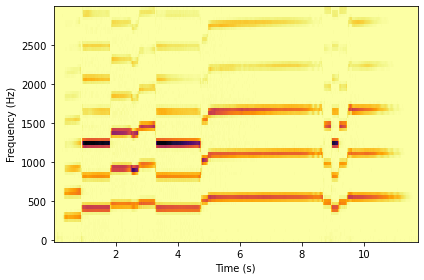
\includegraphics[width=0.8\linewidth]{resources/Images/task4_spectrogram}
        \caption{Спектрограмма записи.}
        \label{fig:task4_spectrogram}
    \end{figure}

    Теперь выберем сегмент записи, отличный от того, с которым происходит работа в примере.

    \begin{lstlisting}[caption= Выбор сегмента и получение его спектра., label={lst:task4_spectrum}]
sax_segment = sax_wave.segment(start=6, duration=0.5)
sax_spectrum = sax_segment.make_spectrum()
sax_spectrum.plot(high=3000)
decorate(xlabel='Frequency (Hz)', ylabel='Amplitude')
sax_segment.make_audio()    \end{lstlisting}

    \begin{figure}[H]
        \centering
        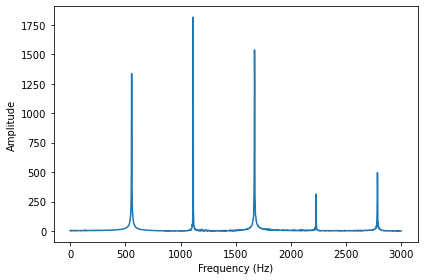
\includegraphics[width=0.7\linewidth]{resources/Images/task4_spectrum}
        \caption{Спектр выбранного сегмента.}
        \label{fig:task4_spectrum}
    \end{figure}

    Теперь узнаем все пики спектра.

    \begin{lstlisting}[caption= Получение пиков спектра., label={lst:task4_peaks}]
sax_spectrum.peaks()[:10]   \end{lstlisting}

    Три наивысших пика находятся на 1114, 1670 и 556 Гц. Из спектра (Рис.\ref{fig:task4_spectrum}) видно, что основная
    частота (556 Гц) не является доминирующей. Хотя именно её мы и воспринимаем. Для сравнения прослушаем звук
    треугольного сигнала с частотой 556 Гц.

    \begin{lstlisting}[caption= Треугольный сигнал с частотой 556 Гц., label={lst:task4_triangle1}]
TriangleSignal(freq=556).make_wave(duration=0.5).make_audio()   \end{lstlisting}

    Если сравнить звук нашего сегмента и созданный треугольный сигнал, можно заметить, что воспринимаемая высота звука
    у них одинаковая.

    Попробуем понять, почему мы воспринимаем основную частоту, даже если она не доминирующая.
    Для этого получим автокорреляционную функцию нашего сегмента.

    \begin{lstlisting}[caption= Функция для получения автокорреляции., label={lst:task4_fun_autocorr}]
def autocorr(segment):
    corrs = numpy.correlate(segment.ys, segment.ys, mode='same')
    N = len(corrs)
    lenght = range(N, N//2, -1)

    half = corrs[N//2:].copy()
    half /= lenght
    half /= half[0]
    return half     \end{lstlisting}

    \begin{lstlisting}[caption= Получение автокорреляционной функции выбранного сегмента., label={lst:task4_autocorr}]
sax_corrs = autocorr(sax_segment)
plt.plot(sax_corrs[:200])
decorate(xlabel='Lag', ylabel='Correlation')    \end{lstlisting}

    \begin{figure}[h]
        \centering
        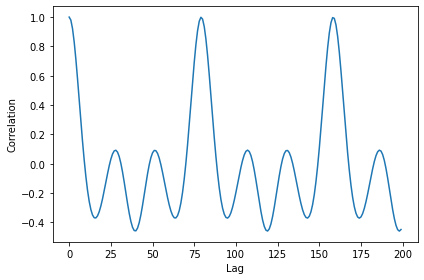
\includegraphics[width=0.7\linewidth]{resources/Images/task4_autocorr}
        \caption{Автокорреляционная функция сегмента.}
        \label{fig:task4_autocorr}
    \end{figure}

    На Рис.\ref{fig:task4_autocorr} видно, что пик находится примерно при lag=75. Уточним это значение и получим
    соответствующую частоту.

    \begin{lstlisting}[caption= Функция для поиска самой высокой корреляции и её частоты., label={lst:task4_fun_find}]
def find_frequency(corrs, low, high):
    lag = numpy.array(corrs[low:high]).argmax() + low
    print(lag)
    period = lag / segment.framerate
    frequency = 1 / period
    return frequency    \end{lstlisting}

    \begin{lstlisting}[caption= Поиск пика и его частоты., label={lst:task4_find}]
find_frequency(sax_corrs, 70, 85)   \end{lstlisting}

    Были получены значения: lag = 79, частота = 558 Гц.

    Таким образом, воспринимаемая высота звука соответствует наивысшему пику автокорреляционной функции, а не
    доминирующей частоте спектра.

    Попробуем убрать основную частоту.

    \begin{lstlisting}[caption= Фильтрация частот ниже 700 Гц., label={lst:task4_spectrum_without_fund}]
sax_spectrum2 = sax_segment.make_spectrum()
sax_spectrum2.high_pass(700)
sax_spectrum2.plot(high=3000)
decorate(xlabel='Frequency (Hz)', ylabel='Amplitude')   \end{lstlisting}

    \begin{figure}[h]
        \centering
        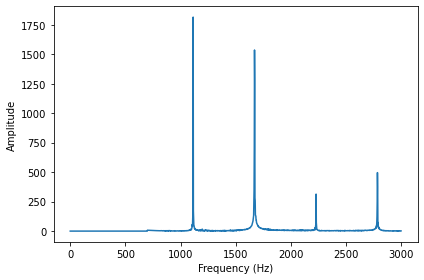
\includegraphics[width=0.8\linewidth]{resources/Images/task4_spectrum_without_fund}
        \caption{Спектр сегмента после фильтрации.}
        \label{fig:task4_spectrum_without_fund}
    \end{figure}

    Преобразуем полученный спектр в \texttt{wave} и прослушаем.

    \begin{lstlisting}[caption= Преобразование в \texttt{wave}., label={lst:task4_wave_without_fund}]
sax_segment2 = sax_spectrum2.make_wave()
sax_segment2.make_audio()   \end{lstlisting}

    Звук, конечно, стал более резким, однако воспринимаемая высота всё ещё совпадает с высотой оригинального сегмента,
    т.е. по прежнему составляет 556 Гц, несмотря на то что на этой частоте нет мощности. Это явление называется
    <<Подавленная основная>>. Этот эффект может использоваться в звуковых системах для расширения области воспроизводимых
    низких частот, если нет возможности адекватно воспроизвести такие частоты напрямую (например, телефоны, наушники).

    Попробуем понять, почему мы всё-таки слышим частоту, которой нет в сигнале. Для этого получим автокорреляционную
    функцию обновлённого сегмента.

    \begin{lstlisting}[caption= Получение автокорреляционной функции обновлённого сегмента., label={lst:task4_autocorr_without_fund}]
sax_corrs = autocorr(sax_segment2)
plt.plot(sax_corrs[:200])
decorate(xlabel='Lag', ylabel='Correlation')    \end{lstlisting}

    \begin{figure}[h]
        \centering
        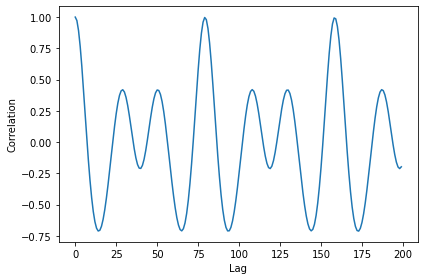
\includegraphics[width=0.8\linewidth]{resources/Images/task4_autocorr_without_fund}
        \caption{Автокорреляционная функция обновлённого сегмента.}
        \label{fig:task4_autocorr_without_fund}
    \end{figure}

    На Рис.\ref{fig:task4_autocorr_without_fund} опять можно наблюдать пик рядом с lag = 75.
    Уточним это значение и получим соответствующую частоту.

    \begin{lstlisting}[caption= Получение частоты пика., label={lst:task4_find_without_fund}]
find_frequency(sax_corrs, 70, 85)   \end{lstlisting}

    И мы вновь получили те же значения: lag = 79, частота = 558 Гц. На Рис.\ref{fig:task4_autocorr_without_fund} можно
    увидеть также ещё два пика: рядом с lag = 25 и lag = 50. Узнаем их частоты.

    \begin{lstlisting}[caption= Получение частот других пиков., label={lst:task4_find_others}]
find_frequency(sax_corrs, 20, 40)
find_frequency(sax_corrs, 40, 60)   \end{lstlisting}

    Были получены частоты 1520 и 882 Гц соответственно. Однако мы всё равно воспринимаем 558 Гц, а не их.
    Это связано с тем, что наивысшие пики, присутствующие в сигнале, являются гармониками 558 Гц, а не 1520 или 882 Гц.
    Наше ухо воспринимает высокие гармоники как подтверждение того, что <<правильной>> основной частотой является
    именно 558 Гц.

    Попробуем избавиться от этих высоких гармоник.

    \begin{lstlisting}[caption= Фильтрация высоких гармоник., label={lst:task4_filter_harmonics}]
sax_spectrum3 = sax_segment.make_spectrum()
sax_spectrum3.high_pass(700)
sax_spectrum3.low_pass(1400)
sax_spectrum3.plot(high=3000)
decorate(xlabel='Frequency (Hz)', ylabel='Amplitude')   \end{lstlisting}

    \begin{figure}[h]
        \centering
        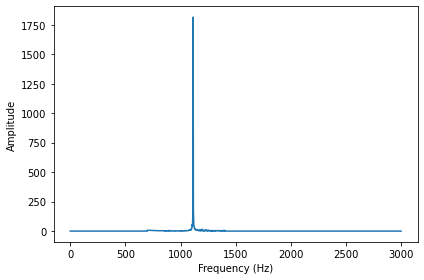
\includegraphics[width=0.8\linewidth]{resources/Images/task4_spectrum_without_harmonics}
        \caption{Спектр сегмента без высоких гармоник.}
        \label{fig:task4_spectrum_without_harmonics}
    \end{figure}

    Теперь преобразуем отфильтрованный спектр в \texttt{wave} и прослушаем результат.

    \begin{lstlisting}[caption= Получение \texttt{wave}., label={lst:task4_filter_harmonics}]
sax_segment3 = sax_spectrum3.make_wave()
sax_segment3.make_audio()   \end{lstlisting}

    Теперь воспринимаемая частота изменилась. Сравним с треугольным сигналом с частотой 1114 Гц.

    \begin{lstlisting}[caption= Треугольный сигнал с частотой 1114 Гц., label={lst:task4_triangle2}]
TriangleSignal(1114).make_wave(duration=0.5).make_audio()   \end{lstlisting}

    Действительно, воспринимаемая высота звука теперь составляет 1114 Гц. Получим автокорреляционную функцию.

    \begin{lstlisting}[caption= Получение автокорреляционной функции., label={lst:task4_autocorr_without_harmonics}]
sax_corrs = autocorr(sax_segment3)
plt.plot(sax_corrs[:200])
decorate(xlabel='Lag', ylabel='Correlation')
    \end{lstlisting}

    Самый высокий пик находится при lag = 40, что соответствует частоте 1102 Гц.

    Таким образом, только удалив основную частоту и её гармоники, мы смогли изменить воспринимаемую высоту звука.
    Это доказывает, что восприятие высоты звука основано на спектральном анализе не полностью, а также определяется
    автокорреляцией.

    \begin{figure}[H]
        \centering
        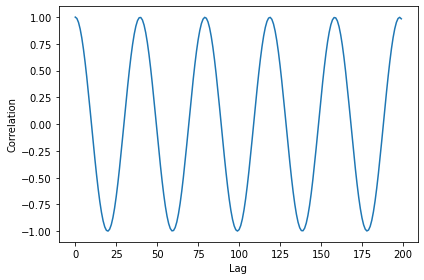
\includegraphics[width=0.8\linewidth]{resources/Images/task4_autocorr_without_harmonics}
        \caption{Автокорреляционная функция сегмента с удалёнными гармониками.}
        \label{fig:task4_autocorr_without_harmonics}
    \end{figure}

    В ходе данного упражнения было изучено явление <<подавленная основная>>, из-за которой воспринимаемая высота тона
    может не меняться, если убрать основную частоту. Кроме того, для избавления от этого эффекта и смены воспринимаемой
    высоты звука были удалены и наивысшие гармоника. Также был сделан вывод, что восприятие высоты звука основано на
    спектральном анализе не полностью, а также определяется автокорреляцией.

    \newpage

% ---------------------------------------------- Выводы ----------------------------------------------
    \section{Выводы}
    \label{sec:conclusions}

    В ходе данной лабораторной работы были изучены возможности автокорреляции для оценки высоты тона звука. Кроме того,
    было исследование <<подавленная основная>>,  из-за которой воспринимаемая высота тона может не меняться, если убрать
    основную частоту. Этот эффект может использоваться для расширения области воспроизводимых низких частот, если
    нет возможности адекватно воспроизвести такие частоты напрямую (например, телефоны и наушники). Был сделан вывод,
    что восприятие высоты звука не полностью основано спектральном анализе, но и определяется автокорреляцией.

\end{document}